\documentclass[main.tex]{subfiles}


\begin{document}
\section{Sum Product Belief Propagation in the 1D Ising Model}


\subsection{Cavity equations}

To find the recursive cavity equations for $\omega_{ i-1 }^{(i)}$ in terms of 
$\omega_{ i-2 } ^{(i-1)}$ we insert Equation (9) from the Exercise sheet into
Equation (8). From this we get expressions for $P^{(i)}(\sigma_{ i-1 } )$ that we
can finally use in Equation (10) to obtain the recursive cavity equations 
\[
    \omega^{i}_{ i-1 } = h + \frac{1}{2\beta} \log( 
    \frac{
        \cosh( \beta  ) + \tanh( \beta \omega_{ i-2 } ^{(i-1)} ) \sinh( \beta )  
    }{
        \cosh( \beta  ) - \tanh( \beta \omega_{ i-2 } ^{(i-1)} ) \sinh( \beta )  
    }
    ) 
.\] 


\subsection*{1.2 \& 1.3\,\, 1D Chain propagation}
Executing the sum product belief propagation algorithm on the 1D chain is very straight forward.
As every site only ever has one other neighbor the cavity precisions propagate along the chain during the algorithm.
For the initial cavity condition we choose $P^{(2)}(\sigma_{ 1 } \pm 1) = \nicefrac{1}{2}$ ($P^{(2)}(\sigma_{ 1 } \pm 1) = \nicefrac{3}{4}$),
which is equivalent to choosing $\omega_{ 1 } ^{2} = 1$ ($\omega_{ 1 } ^{2} = \log( 3 ) $).

\begin{figure}[htpb]
    \centering

    \begin{subfigure}{\textwidth}
        \centering
        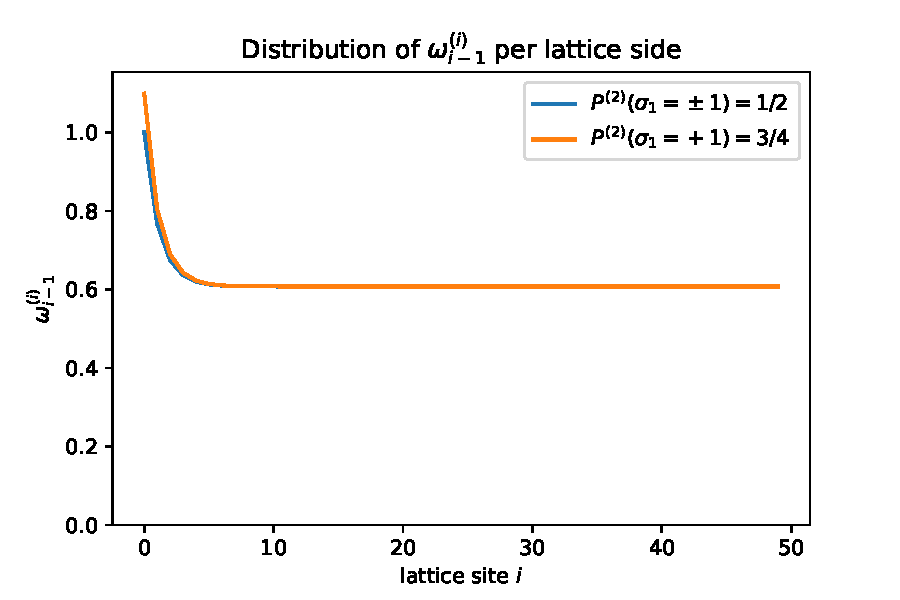
\includegraphics[width=.9\linewidth]{../figures/1_2_precisions.pdf}
        \caption{Solution Ex. 1.2 \& 1.3}
        \label{fig:lattice_precisions_ex}
    \end{subfigure}

    \begin{subfigure}{\textwidth}
        \centering
        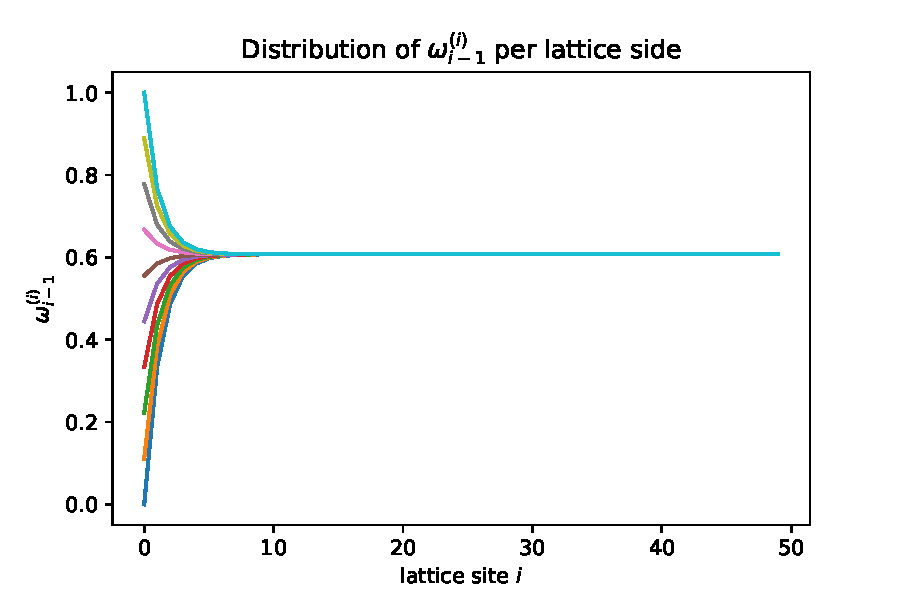
\includegraphics[width=.9\linewidth]{../figures/1_3_precisions.pdf}
        \caption{Qualitative dependence on initial condition}
        \label{fig:lattice_precisions_behavior}
    \end{subfigure} 
    \caption{
        These figures show the cavity precisions $\omega_{ i-1 } ^{(i)}$ on the lattice for different initial cavity conditions.
        In Figure \subref{fig:lattice_precisions_ex} one can see the required solutions to Ex. 1.2 \& 1.3 while in Figure \subref{fig:lattice_precisions_behavior} one can see the cavity precision propagation through the lattice for ten different starting values. 
        This highlights the qualitative behavior of the algorithm.
    }
    \label{fig:lattice_precisions}
\end{figure}

In Figure \ref{fig:lattice_precisions} the behavior of the algorithm is highlighted.
We can see that the initial value does not have an impact on the final value that the algorithm converges against.
This shows that we can find a fixpoint $\omega^{*}$ for given $h$ and $\beta$ that we will use in further analysis of the system.


\subsection*{1.4 \,\,\, Magnetization in Thermodynamic Limit}
In the thermodynamic limit we would expect that the algorithm will indeed converge to a fixpoint as we have seen in Figure \ref{fig:lattice_precisions}.
Due to the workings of the algorithm in the 1D case, to find this fixpoint in our problem we can simply take the cavity precision value of the last site in our chain.

This fixpoint can now be used to calculate the cavity probabilities and from these the actual probabilities.
Such, we can calculate the order parameter of the system, which is the Magnetization $M$  
\[
    \left<M \right> = \frac{1}{N} \sum_{j=1}^{N} \left<\sigma_j \right> \quad\quad
    \text{with} \quad\quad
    \left<\sigma_j \right> = P(\sigma_i = +1) - P(\sigma_i = -1)
.\] 

\begin{figure}[htpb]
    \centering
    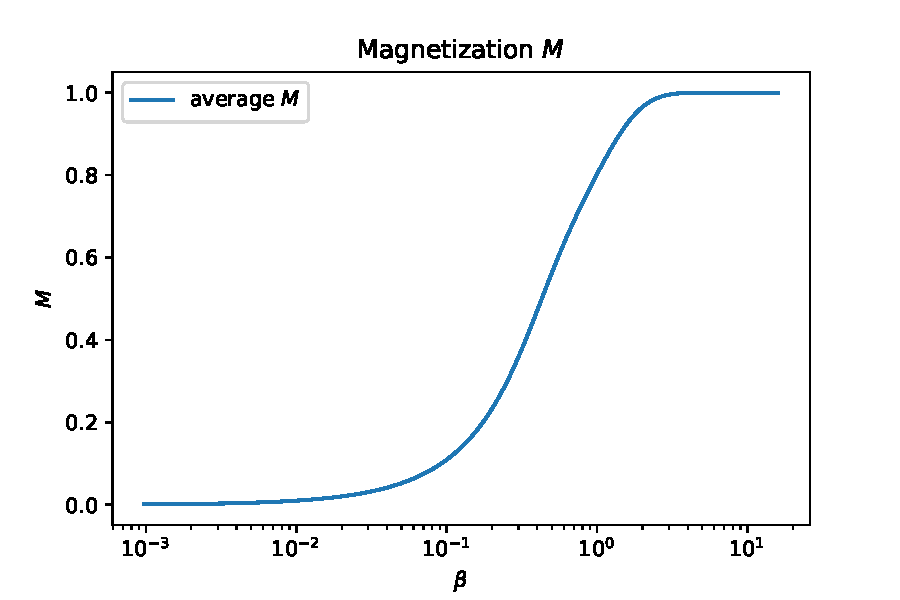
\includegraphics[width=0.8\textwidth]{../figures/1_4_magnetization.pdf}
    \caption{
        This figure shows the average Magnetization of the system plotted against the inverse temperature $\beta$.
        The critical point as given by the theory of phase transition is marked by a red line.
    }
    \label{fig:magnetization}
\end{figure}

In Figure \ref{fig:magnetization} one can see that the average magnetization decreases for higher temperatures (lower $\beta$).
We can also see that the system closely reproduces the critical point of the Ising chain in the thermodynamic limit. 
The reason we can not see the exact behavior is obvious:
Analytical degeneracies can only exist in the thermodynamic limit.
The softening of the phase transition is therefore an expected finite-size effect.


\ifSubfilesClassLoaded{
	% if it's compiled alone
}{
	% if it's compiled in the main file
    \newpage
}
\end{document}
